%Doc
\documentclass[a4paper,12pt]{article}


%Packages
\usepackage[utf8]{inputenc}
\usepackage{amsfonts}
\usepackage[T1]{fontenc}
\usepackage{lmodern}
\usepackage[german]{babel}
\usepackage{amsmath}
\usepackage{amssymb}
\usepackage{mathtools}
\usepackage{setspace}
\usepackage{listings}
\usepackage{color}
\usepackage[left=3cm,right=3cm,top=1cm,bottom=4cm]{geometry}
\usepackage{tikz}
\usepackage{booktabs}

\usetikzlibrary{arrows,automata,positioning}


%Code
\lstset{frame=tb,
  language=Java,
  aboveskip=3mm,
  belowskip=3mm,
  showstringspaces=false,
  columns=flexible,
  basicstyle={\small\ttfamily},
  numbers=none,
  numberstyle=\tiny\color{gray},
  keywordstyle=\color{blue},
  commentstyle=\color{dkgreen},
  stringstyle=\color{mauve},
  breaklines=true,
  breakatwhitespace=true,
  tabsize=3
}
\lstset{literate =%
	{ä}{{\"a}}1
}


%Daten
\author {Daoud Ali 376352, Cihan Orhan 377061\\ Luca Gaudino 379780, Paul Sonnleitner}
\date {}
\title	{\textbf{Softwaretechnik}\\
		Aufgabenblatt \RM{2}
		}


%Commands
\newcommand{\aufgabe}[1]{\section*{Aufgabe #1}}
\newcommand{\apt}[1]{\subsection*{#1)}}
\newcommand{\RM}[1]{\MakeUppercase{\romannumeral #1{}}}


\begin{document}

\doublespacing
\maketitle
\onehalfspacing

\aufgabe{1}
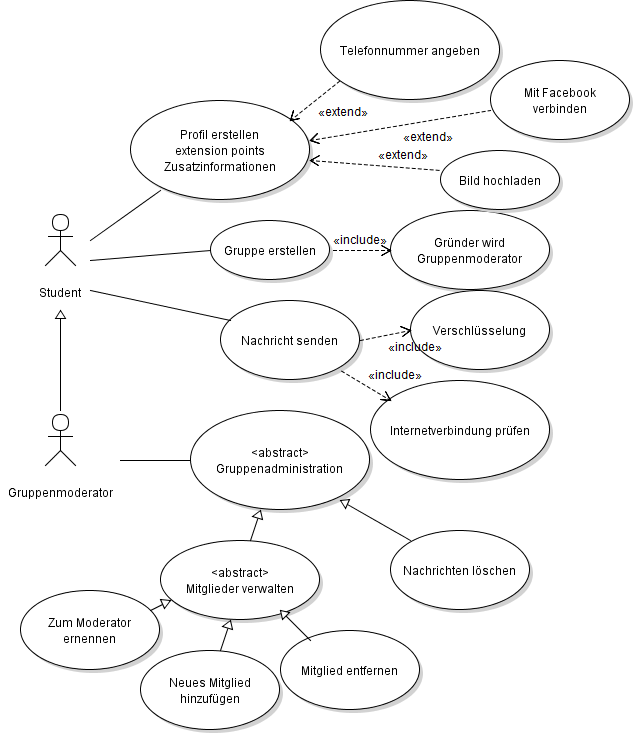
\includegraphics[width=0.7\textwidth]{UseCaseUML_1.png}


\aufgabe{2}
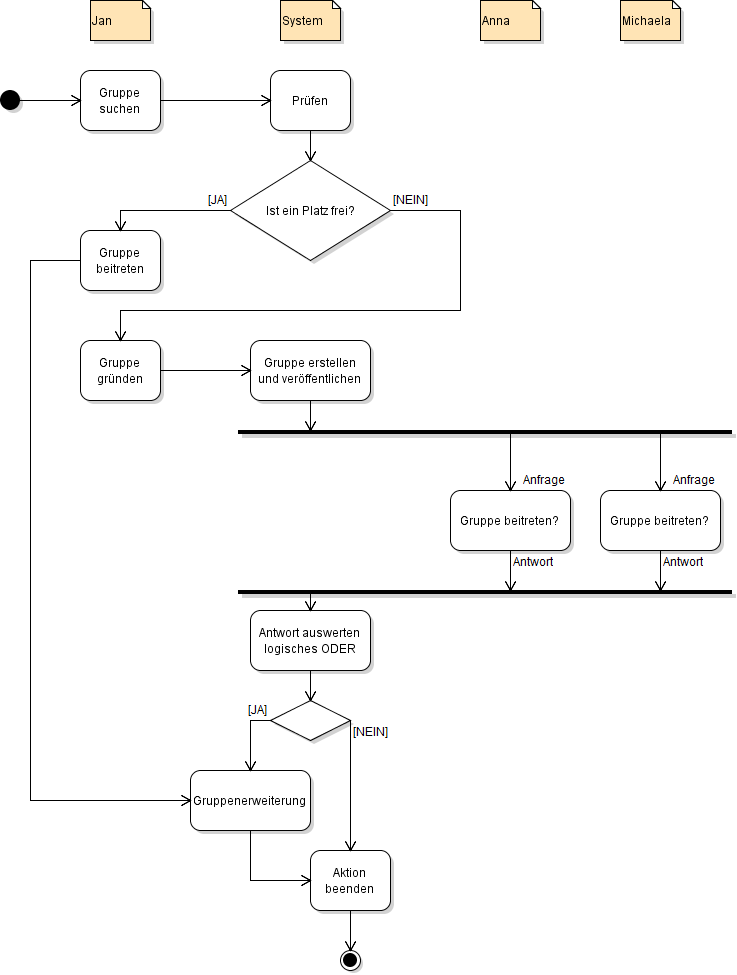
\includegraphics[width=0.7\textwidth]{ActivityUML_1.png}

\end{document}